\documentclass[conference]{IEEEtran}
\usepackage{cite}
\usepackage{amsmath,amssymb,amsfonts}
\usepackage{graphicx}
\usepackage{textcomp}
\usepackage{xcolor}
\usepackage{url}
\usepackage{booktabs}
\usepackage{tikz}
\usetikzlibrary{positioning,arrows.meta}

\begin{document}

\title{Automatic Photo Albums as a Web Service: Content-Based Photo
Grouping with Algorithmically Matched Music}

\author{\IEEEauthorblockN{Jamel Lawson}
\IEEEauthorblockA{\textit{Department of Information Systems} \\
\textit{University of Maryland, Baltimore County}\\
Baltimore, MD \\
jlawson2@umbc.edu}}

\maketitle

\begin{abstract}
I present a web service that turns a set of uploaded photographs
into finished slideshow albums. I describe each photo by simple
visual statistics and by an embedding, a list of numbers produced
by a pre-trained ResNet-50 network that captures what the photo
shows. I group the photos with K-Means clustering, choosing the
number of groups by silhouette score. For each group I build a
cover sheet and pick background music by a fixed rule: I turn the
group's statistics into a target profile, I turn the profile into
a mood-tag search over the Jamendo catalog of Creative Commons
tracks, and a deterministic scoring function picks one track, with
tracks I synthesized in code as a fallback. I then render one
slideshow video per group, timed so the photo changes land on the
beat of the music.
\end{abstract}

\begin{IEEEkeywords}
image clustering, transfer learning, ResNet-50, algorithmic media
selection, Creative Commons music, web services
\end{IEEEkeywords}

\section{Introduction}
Photo collections grow faster than anyone organizes them. A tool
that groups similar photos and presents each group as a short video
album removes the manual sorting step. Two questions follow. How
should similarity be measured so the groups make sense? And when
each album needs background music, how should the music be chosen
so the choice follows a rule anyone can inspect, instead of one
person's taste or a random draw?

I answer both questions with one system. I take similarity from
ResNet-50 embeddings \cite{he2016}: the network was trained on
millions of images, so its embeddings capture shape and content
without any training on the user's photos. I group with K-Means
over those embeddings, and I pick the group count by silhouette
score \cite{rousseeuw1987}, a measure of how well separated the
groups are. I choose music by a documented rule: I turn a
collection's measured brightness, saturation, warmth, and edge
density into a target musical profile, and I let the profile drive
a scored search over a catalog of Creative Commons tracks, with a
small library of tracks I synthesized in code as a fallback. In
the terms of Poole and Mackworth \cite{poole2017}, I built the
service as a simple computational agent: it perceives each upload
through measured features and acts by producing albums, with every
rule fixed in advance and open to inspection.

I began this system as a notebook assignment for a graduate course
on AI agents and deep learning. On a fixed set of 240 licensed
photographs from Wikimedia Commons I scored a cluster purity of
0.821 and a normalized mutual information of 0.739 against the
photos' source topics; both scores say how closely the found
groups match the known topics. In this paper I describe the same
pipeline as a public web service, where a visitor uploads 8 to 240
photos and receives covers, music, and slideshow videos for every
collection the system finds.

\section{System Design}

Figure \ref{fig:pipeline} shows the pipeline I built, end to end.
I fixed every stage's rules in advance, and I store the numbers
each stage produces with the job, so I can explain every output
afterwards.

\begin{figure*}[htbp]
\begin{center}
\resizebox{\textwidth}{!}{%
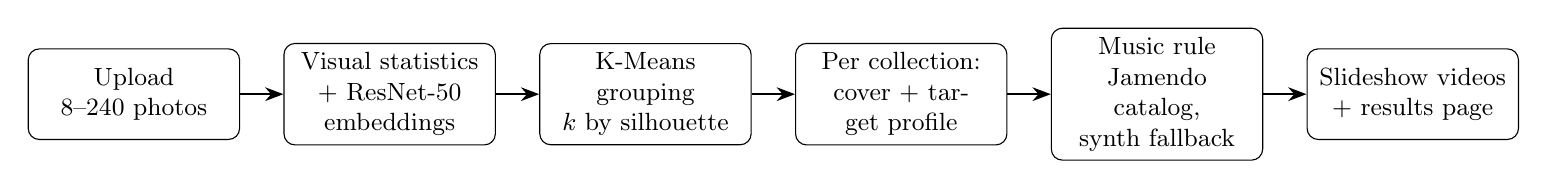
\begin{tikzpicture}[
  box/.style={draw, rounded corners, align=center, font=\small,
              text width=2.45cm, minimum height=1.15cm},
  arrow/.style={-{Stealth}, thick}]
\node[box] (up) {Upload\\8--240 photos};
\node[box, right=0.55cm of up] (feat) {Visual statistics\\+ ResNet-50 embeddings};
\node[box, right=0.55cm of feat] (km) {K-Means grouping\\$k$ by silhouette};
\node[box, right=0.55cm of km] (cov) {Per collection:\\cover + target profile};
\node[box, right=0.55cm of cov] (mus) {Music rule\\Jamendo catalog,\\synth fallback};
\node[box, right=0.55cm of mus] (vid) {Slideshow videos\\+ results page};
\draw[arrow] (up) -- (feat);
\draw[arrow] (feat) -- (km);
\draw[arrow] (km) -- (cov);
\draw[arrow] (cov) -- (mus);
\draw[arrow] (mus) -- (vid);
\end{tikzpicture}}
\caption{The album pipeline, from upload to finished slideshows.}
\label{fig:pipeline}
\end{center}
\end{figure*}

\subsection{Visual statistics}
I shrink each photo to a $128 \times 128$ thumbnail, and I compute
four statistics: brightness, saturation, warmth (red minus blue),
and edge density (how much detail the photo has). A three-center
K-Means over sampled pixels gives three dominant colors. These
statistics are cheap to compute and easy to explain, and I use
exactly these statistics in the music rule.

\subsection{Feature extraction}
I embed each photo with ResNet-50 pre-trained on ImageNet
\cite{deng2009}, with the classification head removed so I keep
the 2,048-number pooled feature. I normalize embeddings to unit
length, which makes plain K-Means group by similarity of content.
Pre-trained features are the right choice here because I must
handle any photos a visitor uploads, with no training set of my
own.

\subsection{Clustering}
I try K-Means for each candidate group count $k$ in a range set by
the number of photos, and I keep the $k$ with the best silhouette
score. For the original assignment dataset I could score the
groups against the photos' known topics; for a visitor's upload I
have no ground truth, so I report the silhouette score I used and
describe each collection by its size, its dominant colors, and its
average statistics.

\subsection{Music sources and the selection rule}
I scale each collection's statistics across the run into a target
profile with five numbers: tempo, mode, timbre, register, and
warmth. Edge density sets the tempo; brightness and saturation set
the mode, register, and timbre; warmth carries over. I drive two
music sources from the profile.

The primary source is the Jamendo catalog of Creative Commons
music, which I search through its public API. I turn the target
into search tags: a bright target gives happy and uplifting tags,
a dark one melancholic and dramatic ones; a warm target adds
acoustic and folk, a cool one electronic and ambient; very fast or
slow targets add energetic or relaxing. I then score each
candidate track by a fixed rule: how close its rated speed is to
the target tempo, how many of the search tags it carries, whether
it can be downloaded, and its track identifier as a tie-break. Two
practical findings shaped my design. Most catalog tracks have no
speed rating, so the API's own speed filter returns almost
nothing; I score speed locally when present and ignore it when
absent. And a tag search can come back empty, so I retry with
fewer tags before giving up. I download the winning track, and I
show its title, artist, catalog page, and Creative Commons licence
on the results page.

The fallback source is four original tracks (calm, bright, warm,
dramatic) that I synthesized with NumPy: chord pads, a bass line,
and a seeded melody, at tempos from 72 to 116 BPM. Each carries
the same five-number profile, and I pick the track closest to the
target by a weighted distance. I run the fallback when no API key
is set, the API is unreachable, or no candidate survives. Either
way I keep the choice deterministic: the same photos always get
the same music, and I store every score so the choice can be
checked later.

\subsection{Slideshow generation}
For each collection's slideshow I use up to twelve photos nearest
the collection's center. I place every photo on a $1280 \times
720$ canvas over a blurred enlargement of itself, so I crop
nothing. I mix the collection's track in as audio, and I encode
the video as H.264 with ffmpeg. Figure \ref{fig:frame} shows one
frame; the full video is at
\url{https://drive.google.com/file/d/1i85gaqTzuXiqpCSvA3wFZmRBnSUAeHzE/view}.

I make the photo changes follow the beat of the music. A beat
module I wrote estimates the track's tempo and beat positions from
its onset pattern, gives each photo a whole number of beats (about
2.6 seconds' worth), and places each fade so it lands exactly on a
beat. When I find no reliable beat, as with near-silent audio, I
keep fixed 2.6-second timing. The module uses only NumPy, so I add
no new dependency.

\begin{figure}[htbp]
\begin{center}
\includegraphics[width=\columnwidth]{slideshow_frame.jpg}
\caption{A frame from a generated slideshow video (mountains
collection), showing the blurred-fill canvas.}
\label{fig:frame}
\end{center}
\end{figure}

\subsection{Web architecture}
I built the service as a Flask application. I store an upload as a
job, convert it to JPEG at intake (including HEIC, the iPhone
format), and process it in a background thread while the browser
polls a status page; the results page then shows each collection's
cover, statistics, track with an audio player, and video. I take 8
to 240 photos, and I offer a built-in example run over the same
240 seed photos as the notebook run for visitors who do not want
to upload their own. I deploy the hosted service as an add-on to
the same pipeline; the full 240-image assignment run lives in the
companion notebook. I run it on Render on a 2 GB instance, because
smaller tiers run out of memory during feature extraction.

One intake detail mattered in practice. Phone cameras store
portrait photos as landscape pixels plus an orientation tag in the
photo's EXIF data, and the imaging library ignores that tag when
it re-saves a file. My first deployed version therefore turned
portrait photos sideways in the covers and videos. I now apply the
EXIF orientation at intake before re-encoding, and I apply it
again wherever the pipeline opens a photo, so a portrait stays
portrait end to end; two regression tests cover the case.

\section{Implementation and Code Analysis}
I wrote the code as five Python modules: \texttt{app.py} (routes,
jobs, and page templates, 668 non-comment lines),
\texttt{pipeline.py} (statistics, embeddings, clustering, covers,
video, 230 lines), \texttt{music.py} (synthesis and the fallback
rule, 145 lines), \texttt{jamendo.py} (catalog search, scoring,
download, 102 lines), and \texttt{beats.py} (beat analysis and
timing, 116 lines). Figure \ref{fig:tree} shows the repository
layout. Tables \ref{tab:cloc} and \ref{tab:lizard} summarize a
CLOC count and a Lizard complexity analysis of the modules and the
tests.

\begin{figure}[htbp]
\footnotesize
\begin{verbatim}
photo-albums-app/
+-- app.py          Flask routes, jobs
+-- pipeline.py     statistics, embeddings,
                    clustering, covers, video
+-- music.py        synthesized tracks,
                    fallback selection rule
+-- jamendo.py      catalog search, scoring,
                    download, attribution
+-- beats.py        beat analysis, segment
                    timing on the beat grid
+-- data/           example set manifest
                    (240 seed photos)
+-- requirements.txt
+-- render.yaml     Render deployment
+-- tests/          33 unit tests
+-- docs/           CLOC and Lizard outputs
+-- jobs/           one folder per upload
                    (created at runtime)
\end{verbatim}
\caption{Repository layout of the web service.}
\label{fig:tree}
\end{figure}

\begin{table}[htbp]
\caption{CLOC count (cloc 2.06), application and tests}
\begin{center}
\begin{tabular}{lrrrr}
\toprule
Language & Files & Blank & Comment & Code \\
\midrule
Python & 11 & 268 & 615 & 1084 \\
\bottomrule
\end{tabular}
\label{tab:cloc}
\end{center}
\end{table}

\begin{table}[htbp]
\caption{Lizard analysis of the application modules}
\begin{center}
\begin{tabular}{lrrrr}
\toprule
File & NLOC & Functions & Avg NLOC & Avg CCN \\
\midrule
app.py & 668 & 16 & 8.8 & 2.8 \\
pipeline.py & 230 & 10 & 22.0 & 4.8 \\
music.py & 145 & 9 & 11.6 & 2.8 \\
jamendo.py & 102 & 8 & 11.4 & 4.8 \\
beats.py & 116 & 8 & 13.8 & 3.9 \\
\textbf{Total} & \textbf{1261} & \textbf{51} & \textbf{13.0} & \textbf{3.7} \\
\bottomrule
\end{tabular}
\label{tab:lizard}
\end{center}
\end{table}

Lizard raises one warning: the orchestration function
\texttt{run\_pipeline} has a cyclomatic complexity of 22 against a
threshold of 15. The complexity comes from the stages it runs in
sequence rather than from nested logic; I recorded splitting out
the per-collection cover and video stages as the first refactoring
candidate in the project's analysis notes. Most of
\texttt{app.py}'s line count is its embedded page templates.

\section{Evaluation}
I cover the system with thirty-three unit tests: the music
profiles and synthesis, the selection rule and its tie-breaks, the
visual statistics, recovery of a known group count from synthetic
embeddings, the web routes, the catalog module and its fallbacks,
and the beat module (tempo and beat recovery on synthetic tracks,
no beat for silence, and the timing planner's rules), plus two
regression tests that portrait photos keep their orientation. All
thirty-three pass in about ten seconds.

For the full assignment run, which I executed in the notebook, I
used the fixed dataset of 240 photographs: 30 each from eight
topics (mountains, beach, city, forest, desert, snow, dogs, and
flowers), all from Wikimedia Commons, with creator and license
recorded in the dataset manifest. The silhouette score peaked at
$k = 8$ (0.150, against 0.144 at $k = 7$ and 0.143 at $k = 9$); I
also scored a second method, agglomerative clustering, at 0.147 at
the same $k$. Against the known topics, the eight collections
scored a purity of 0.821 and a normalized mutual information of
0.739. Five of the eight collections were at least 90 percent one
topic; the mixing concentrated in the forest, mountains, and snow
collections, whose topics share texture and color. I built
slideshow videos for the three largest collections.

I ran the web service end to end twice with 24 photos spanning
four topics. With the synthesized library, it chose $k = 4$
(silhouette 0.159), produced collections of 7, 5, 6, and 6 photos,
picked the warm track twice and the calm track twice, and rendered
four videos; I verified each as H.264 video with AAC audio. With
the catalog enabled, all four collections received real Creative
Commons tracks: \textit{plaid shirt (revisited)} by Ton,
\textit{Life is good} by Galdson, \textit{Breathe} by Axl \&
Arth, and \textit{Energy} by Pokki DJ. Four collections that had
shared two synthesized tracks now carried four distinct recorded
songs, each traceable to the profile that selected it.

I checked beat timing in a further run of the same photos. My
analyzer measured all four tracks, at 104.8, 143.8, 124.6, and
128.3 BPM; one synthesized track plays its melody on eighth notes,
so its measured grid is the eighth-note grid, and changes still
land on note onsets. Each video's measured length matched its
planned beat total within about a tenth of a second. I also
verified the built-in example run live: it fetched all 240 seed
photos, chose $k = 8$ with silhouette 0.15, and produced eight
beat-timed collections, five with catalog tracks and three with
synthesized ones.

\subsection{Walkthrough of the hosted service}
Figures \ref{fig:wt-home} to \ref{fig:wt-results} walk through one
live run I made with the same 24 photos. The upload page
(Fig. \ref{fig:wt-home}) takes the photos and starts the job. The
status page (Fig. \ref{fig:wt-working}) reports each stage as it
finishes, here caught during the music stage. The results page
(Fig. \ref{fig:wt-results}) shows every collection with its cover,
statistics, matched track with the search the rule ran, and its
video. In this run three collections received catalog tracks and
one used the synthesized library, so the walkthrough shows both
music paths as a visitor sees them.

\begin{figure}[htbp]
\begin{center}
\includegraphics[width=\columnwidth]{walkthrough_home.jpg}
\caption{The upload page of the hosted service.}
\label{fig:wt-home}
\end{center}
\end{figure}

\begin{figure}[htbp]
\begin{center}
\includegraphics[width=\columnwidth]{walkthrough_working.jpg}
\caption{The status page during a run, with the music stage in
progress and the video stage still pending.}
\label{fig:wt-working}
\end{center}
\end{figure}

\begin{figure}[htbp]
\begin{center}
\includegraphics[width=\columnwidth]{walkthrough_results.jpg}
\caption{The top of the results page: run summary and the first
collection's cover sheet and statistics.}
\label{fig:wt-results}
\end{center}
\end{figure}

\section{Limitations}
K-Means favors round, similarly sized groups, so a collection with
one main subject and many outliers can split awkwardly. Catalog
metadata is uneven: many tracks have no speed rating and tag
wording varies by uploader, so my matches are only as precise as
the catalog's own descriptions. I kept the synthesized tracks
deliberately simple; in both sources my contribution is the
selection rule, not the composition. I run processing on CPU, so
large uploads take minutes, and I store job results on the
service's local disk, where they do not survive redeploys.

\section{Conclusion}
A course pipeline for grouping photos and choosing music by rule
carries over cleanly to a public web service. The pieces that made
my original system defensible, measured statistics, a documented
selection rule, and stored scores, are the same pieces that make
the hosted version explainable: every album can say why its photos
are together and why the rule picked its music.

\section*{Artifact Availability}
I collected all of the artifacts here. The executed Jupyter
notebook with the full 240-image run opens in Google Colab at
\url{https://colab.research.google.com/github/jamelski1/seng691-hw5/blob/main/seng691-hw5.ipynb};
I keep its source repository, including the dataset manifest, at
\url{https://github.com/jamelski1/seng691-hw5}. The dataset is
public: the manifest listing all 240 photographs with their
creators, licenses, and Wikimedia Commons source pages is at
\url{https://github.com/jamelski1/photo-albums-app/blob/main/data/example_manifest.csv}.
A generated slideshow
video is on Google Drive at
\url{https://drive.google.com/file/d/1i85gaqTzuXiqpCSvA3wFZmRBnSUAeHzE/view}.
The web service source is at
\url{https://github.com/jamelski1/photo-albums-app}, and the running
service is at \url{https://photo-albums-y7ir.onrender.com}.

\section*{AI Use Disclosure}
I used AI assistants (Claude and Llama) during development of
the web service, including implementation and testing support.
I executed and verified all code, and every reported result
comes from those verified runs.

\begin{thebibliography}{00}
\bibitem{he2016} K. He, X. Zhang, S. Ren, and J. Sun, ``Deep residual
learning for image recognition,'' in \textit{Proc. IEEE Conf. Comput.
Vis. Pattern Recognit.}, 2016, pp. 770--778.
\bibitem{deng2009} J. Deng, W. Dong, R. Socher, L.-J. Li, K. Li, and
L. Fei-Fei, ``ImageNet: A large-scale hierarchical image database,''
in \textit{Proc. IEEE Conf. Comput. Vis. Pattern Recognit.}, 2009,
pp. 248--255.
\bibitem{rousseeuw1987} P. J. Rousseeuw, ``Silhouettes: A graphical
aid to the interpretation and validation of cluster analysis,''
\textit{J. Comput. Appl. Math.}, vol. 20, pp. 53--65, 1987.
\bibitem{poole2017} D. L. Poole and A. K. Mackworth,
\textit{Artificial Intelligence: Foundations of Computational
Agents}, 2nd ed. Cambridge, U.K.: Cambridge University Press, 2017.
\end{thebibliography}

\end{document}
